\documentclass[journal]{IEEEtran}
\usepackage[utf8]{inputenc}

\usepackage{array}
\usepackage[backend=biber]{biblatex}
\usepackage{graphicx}
\usepackage{hyperref}
\usepackage{siunitx}
\usepackage{tabu}

\addbibresource{references.bib}
 
\hypersetup{
    colorlinks=true,
    linkcolor=blue,
    filecolor=magenta,      
    urlcolor=cyan,
}

% correct bad hyphenation here
\hyphenation{Watts-Strogatz net-works measure-ments}

% - - - - - - - - - - - - - - - - - - - - - - - - - - -

\begin{document}

\title{Defining and computing entropy for networks}

\author{
Henrique Ferrolho - s1683857,
Team: Alex Hoppen, Charles Desmonty
}

% make the title area
\maketitle

% - - - - - - - - - - - - - - - - - - - - - - - - - - -

\begin{abstract}

We will define two different measures to calculate the entropy of a graph network, i.e. its level of disorder. Both these measurements will use very basic properties of the graph's structure itself.

We will run test trials on these measurements with \textit{Erdős-Rényi} and \textit{Watts-Strogatz} random graphs. Furthermore, we will run more trials using real-world datasets of very large road networks.

Finally, we will introduce the concept of \textit{Kolmogorov Complexity}, and suggest an approach that can be used as a different entropy measurement for future works.

\end{abstract}

% - - - - - - - - - - - - - - - - - - - - - - - - - - -

\section{Introduction}

Entropy is the lack of \textit{order} or \textit{predictability}, it is a measure of \textit{randomness} or \textit{disorder} in a system - the greater the disorder the higher the entropy.

We are going to define a measure in order to calculate the entropy of a network graph. But before we do that, we need to agree on what makes a network more or less organized. How does the human notion of order apply to graphs, i.e. having two graphs $A$ and $B$, what properties make graph $A$ more or less organized and structured than graph $B$?

Entropy must be carefully defined both as a measure and as a concept.

\bigskip

In this paper we will briefly go through related works on the subject from the past.

Furthermore, we will define two different definitions for entropy of a graph.

We will then proceed to test them not only on two types of random graphs: \textit{Erdős-Rényi} graphs \cite{erdosRenyiGraphs}, and \textit{Watts-Strogatz} graphs \cite{watts1998collective}, but also on two real-world road network datasets \cite{snapnets}.

% - - - - - - - - - - - - - - - - - - - - - - - - - - -

\section{Related work}

Trying to come up with a robust definition for the entropy of a graph has been an extensively explored topic during the past: Dehmer \cite{dehmer2008} and \cite{dehmer2011}.

Zenil and Kiani \cite{zenil2016low} have explained how information-theoretic measures are not independent of the way in which a graph can be observed. They explore Shannon Entropy as a computable measure, and introduce recursive and non-recursive uncomputable graphs to demonstrate the weaknesses of measures of complexity.

% - - - - - - - - - - - - - - - - - - - - - - - - - - -

\section{Graph entropy}

\subsection{Notation}

Let $ \mathcal{G} = (V, E) $ be a graph where $V$ is the set of \textit{nodes} and $E$ the set of \textit{edges}. Furthermore, let \textit{deg($v$)} denote the \textit{degree} of a node $v \in V$, and \textit{avg\_deg($V$)} the average degree of the graph's node set.

\begin{equation}
   avg\_deg(V) =  \frac{1}{|V|} \sum_{v \in V} deg(v)
\end{equation}

Let $C(V)$ be the subset of nodes in $V$ that have a degree greater than 0. Then, let $ distinct(C(V)) $ denote the number of distinct values in $C(V)$.

We are now going to define two different ways to calculate the entropy of a graph: $\mathcal{H}1(\mathcal{G})$ and $\mathcal{H}2(\mathcal{G})$.

The entropy $\mathcal{H}1$ of a graph $\mathcal{G}$ is given by the quotient of the distinct number of node degrees in the set minus one, and the total number of nodes in the graph.

\begin{equation}
   \mathcal{H}1(\mathcal{G}) = \frac{distinct(C(V)) - 1}{|V|}
\end{equation}

\bigskip

The entropy $\mathcal{H}2$ of a graph $\mathcal{G}$ is the quotient of the square root of the summation of the a node's degree variance, and the total number of nodes in the graph. $\mathcal{H}2$ is given by the following equation:

\begin{equation}
   \mathcal{H}2(\mathcal{G}) = \frac{1}{|V|} \sqrt{\sum_{v \in V} [deg(v) - avg\_deg(V)] ^ 2}
\end{equation}

\subsection{Applying H1 to a complete graph}

Let $\mathcal{G}1$ be a complete graph with 6 nodes ($|V| = 6$). Then, \texttt{nx.degree\_histogram($\mathcal{G}1$)} = [0, 0, 0, 0, 0, 6], $ distinct(C(V)) = 1$, and finally $\mathcal{H}1(\mathcal{G}1) = (1 - 1) / 6 = 0$

\begin{figure}[ht]
    \centering
    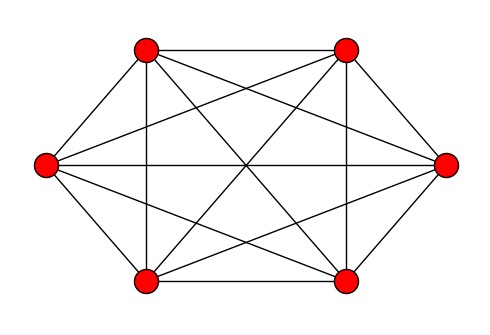
\includegraphics[width=0.6\linewidth]{res/complete-graph.png}
    \caption{A complete graph with 6 nodes. Each node is connected to every other node in the graph. $\mathcal{H}1$ classifies it as having entropy 0.
    }
\end{figure}

% - - - - - - - - - - - - - - - - - - - - - - - - - - -

\section{Results}

In this section we present results for $\mathcal{H}1$ and $\mathcal{H}2$ on random graphs with $n = 500$ and $n = 1000$. These were obtained by running Jupyter Notebooks that can be found at \url{https://github.com/ferrolho/uoe-stn}.

\bigskip

By analysing figures 2 to 5, we can see that both measurements $\mathcal{H}1$ and $\mathcal{H}2$ are robust, and all the plots look very similar, whether or not the number of nodes $n$ of the graph changed.

\bigskip

On all the experiments it can be observed that the entropy of \textit{Erdős-Rényi} graphs tend to zero whether $p$ tends to 0 or 1. Furthermore, the entropy measurement $\mathcal{H}1$ seems to differ only from $\mathcal{H}2$ by a constant.

\bigskip

\begin{figure}[ht]
    \centering
    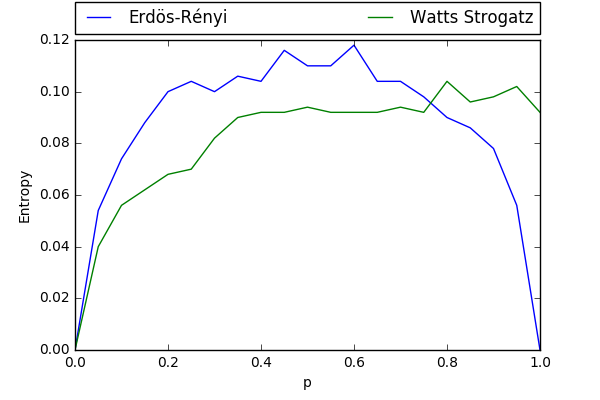
\includegraphics[width=\linewidth]{res/entropy1/experiment_n500.png}
    \caption{$\mathcal{H}1$ results on random graphs with $n = 500$.}
\end{figure}

\begin{figure}[ht]
    \centering
    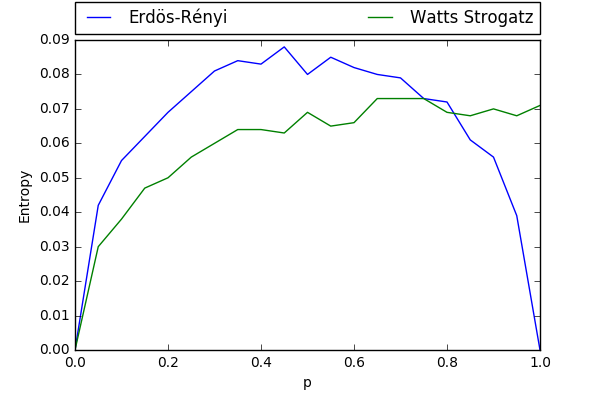
\includegraphics[width=\linewidth]{res/entropy1/experiment_n1000.png}
    \caption{$\mathcal{H}1$ results on random graphs with $n = 1000$.}
\end{figure}

Regarding \textit{Watts Strogatz} graphs, it behaves differently from \textit{Erdős-Rényi} graphs as the probability $p$ increases. But it is consistent as to being 0 when $p$ tends to 0. And just like \textit{Erdős-Rényi} graphs, measurement $\mathcal{H}1$ and $\mathcal{H}2$ seem to differ only by a constant.

To sum up the experimental results on random graphs: we ran multiple trials for the two measurements we defined, and we varied the number of nodes of the random graphs on the test trials. The results seem to suggest that no matter what the number of nodes in the graph is, both entropy measurements stand robust and output very similar results, differing only by a product constant.

Therefore, the results seem to imply that both $\mathcal{H}1$ and $\mathcal{H}2$ are measuring the same properties of graphs, even though they have very different equations. If this is correct, and $\mathcal{H}1$ is indeed an approximation of $\mathcal{H}2$, then the first should be preferred over the latter because its computational complexity is remarkably simpler.

\begin{figure}[ht]
    \centering
    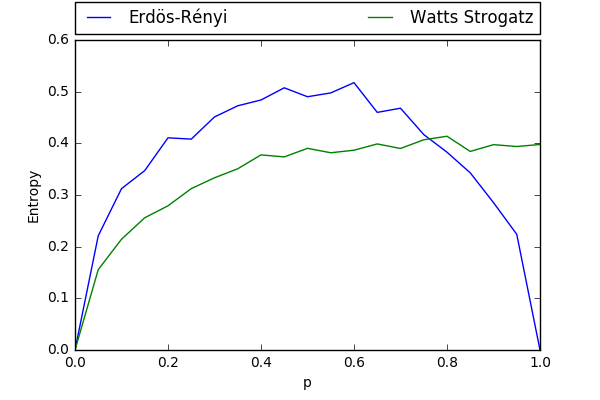
\includegraphics[width=\linewidth]{res/entropy2/experiment_n500.png}
    \caption{$\mathcal{H}2$ results on random graphs with $n = 500$.}
\end{figure}

\begin{figure}[ht]
    \centering
    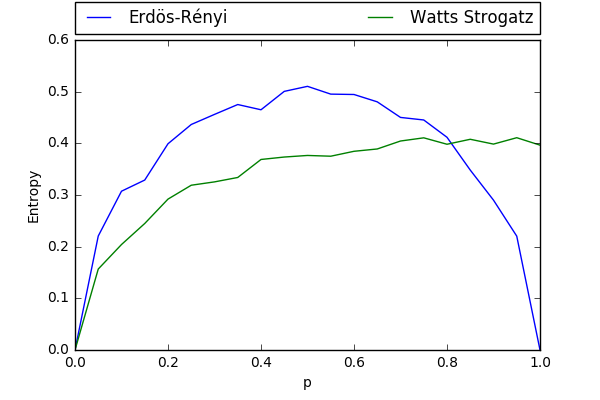
\includegraphics[width=\linewidth]{res/entropy2/experiment_n1000.png}
    \caption{$\mathcal{H}2$ results on random graphs with $n = 1000$.}
\end{figure}

\subsection{Real-world datasets}

We now turn into real-world dataset results from SNAP \cite{snapnets}. We used two datasets: a road network of California, and of Texas. These datasets contain intersections that are represented by nodes, and roads connecting these intersections which are represented by undirected edges.

\bigskip

We implemented a simple Python program to parse each dataset, load the information to  NetworkX graph, and to calculate the entropy of each one using our two different measurements. This program can also be found at \url{https://github.com/ferrolho/uoe-stn}.

\bigskip

The following table shows the number of nodes and the number of edges on each of the road network datasets.

\bigskip

\begin{table}[ht]
    \centering
	\begin{tabu} to 0.45\textwidth{ | X[c] | X[c] | X[c] | }
		\hline
		& & \\
		Dataset & Nodes & Edges \\
		& & \\
		\hline
		& & \\
		roadNet-CA & 1965206 & 2766607 \\
		& & \\
		roadNet-TX & 1379917 & 1921660 \\
		& & \\
		\hline
	\end{tabu}
	\medskip
    \caption{Table with the number of nodes and the number of edges on each of the road network datasets.}
\end{table}

As we had previously suspected, the calculation of the graphs' entropy using $\mathcal{H}1$ was much faster and less costly compared to the entropy measurement $\mathcal{H}2$.

\begin{table}[ht]
    \centering
	\begin{tabu} to 0.45\textwidth{ | p {0.12\textwidth} | p {0.12\textwidth} | X[c] | X[c] | }
		\hline
		& & & \\
		Entropy 1 & Entropy 2 & Time 1 & Time 2 \\
		& & & \\
		\hline
		& & & \\
		$2.54 \times 10^{-6}$ & $501.70 \times 10^{-6}$ & \SI{5.75}{\s} & \SI{57.68}{\s} \\
		& & & \\
		$2.90 \times 10{^-6}$  & $605.23 \times 10^{-6}$  & \SI{3.42}{\s} & \SI{40.05}{\s} \\
		& & & \\
		\hline
	\end{tabu}
	\medskip
    \caption{Table with the trials' results: top line is in respect to California, bottom line is in respect to Texas.}
\end{table}

The entropy values are also compatible with the results of the test trials using \textit{Erdős-Rényi} and \textit{Watts Strogatz} random graphs.

Finally, we can conclude that the Texas road network is slightly more disordered than California, since it has a greater entropy.

\bigskip

% - - - - - - - - - - - - - - - - - - - - - - - - - - -

\appendices

\section{Kolmogorov complexity}

The \textit{Kolmogorov complexity} \cite{li2009introduction} of an object is the length of the shortest program that outputs that same object.

\bigskip

One can think of \textit{entropy} as an indicator of disorder, but it is also valid to think of it as the predictability of a system, or even more: the amount of information required to describe a system exactly as is.

\bigskip

Therefore, it might be interesting to try and come up with a measurement of the entropy of a graph with respect to the \textit{Kolmogorov complexity}.

For example, if two distinct graphs - $A$ and $B$ - can be represented with the same \textit{Kolmogorov complexity}, i.e. a minimal representation with the same length, than it is only reasonable to think of them as having the same level of entropy.

\bigskip

% - - - - - - - - - - - - - - - - - - - - - - - - - - -

\printbibliography

\end{document}
